%%%%%%%%%%%%%%%%%%%%%%%%%%
%% Folie: Background    %%
%%%%%%%%%%%%%%%%%%%%%%%%%%
\begin{frame}
    \frametitle{Background -- RANS}
 TODO
\end{frame}
\clearpage

%%%%%%%%%%%%%%%%%%%%%%%%%%
%% Folie: Background    %%
%%%%%%%%%%%%%%%%%%%%%%%%%%
\begin{frame}
    \frametitle{Background -- Convolutions}
\vspace*{5mm}
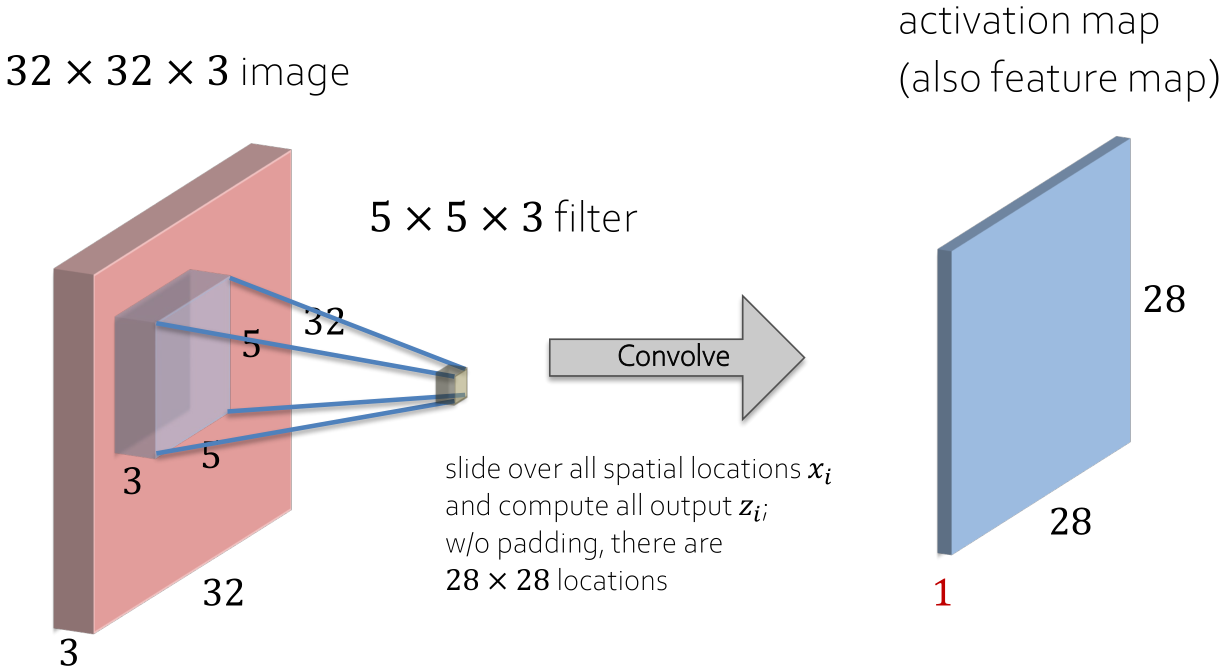
\includegraphics[width=0.8\textwidth, height=.55\textheight]{./Ressourcen/Praesentation/Bilder/conv_bsp.png}%

Taken from I2DL WS19/20 (TUM)
    
\end{frame}
\clearpage

%%%%%%%%%%%%%%%%%%%%%%%%%%
%% Folie: Background    %%
%%%%%%%%%%%%%%%%%%%%%%%%%%
\begin{frame}
    \frametitle{Background -- Convolutions}

Low-Level Features, Mid-Level Features, High-Level Features: each filter captures different characteristics

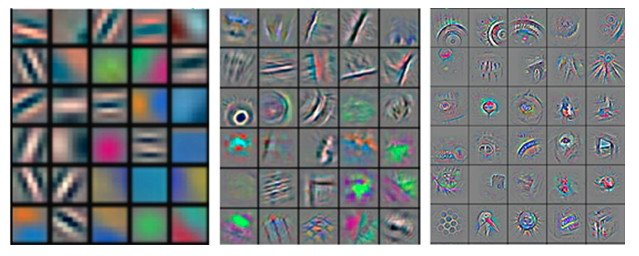
\includegraphics[width=0.8\textwidth, height=.55\textheight]{./Ressourcen/Praesentation/Bilder/features.png}%
\vspace*{-5mm}

Taken from \url{https://arxiv.org/pdf/1311.2901.pdf}   
    
\end{frame}
\clearpage